
\documentclass{article}
\usepackage{hyperref}
\usepackage{enumitem}
\usepackage{graphicx}
\usepackage{amsmath}
\usepackage{mathpazo}
\usepackage{xcolor}
\usepackage{float}
\usepackage{listings}
\lstset{
  basicstyle=\ttfamily\small,
  breaklines=true,
  columns=fullflexible,
  frame=single,
  showspaces=false,
  showtabs=false,
  keepspaces=false
}
\usepackage[export]{adjustbox}
\usepackage{multicol}
\usepackage{caption}
\usepackage[a4paper,
            bindingoffset=0.2in,
            left=0.5in,
            right=0.5in,
            top=0.5in,
            bottom=0.5in,
            footskip=.25in]{geometry}


\begin{document}
\title{MS Technical Paper: \\ Placement Algorithms for Heterogeneous FPGAs}
\author{Brian B Cheng \\ Rutgers University Department of Electrical and Computer Engineering}


\date{}
\maketitle

\begin{multicols}{2}

\section{Keywords}
\begin{itemize}
    \item FPGA, EDA, Placement, Simulated Annealing, Optimization, RapidWright
\end{itemize}


\section{Abstract}
    fdsafdsafdsa. \\ 
    fdsafdsafdsa. \\ 
    fdsafdsafdsa. \\ 
    fdsafdsafdsa. \\ 
    fdsafdsafdsa. \\ 
    fdsafdsafdsa. \\ 
    fdsafdsafdsa. \\ 
    fdsafdsafdsa. \\ 
    fdsafdsafdsa. \\ 
    fdsafdsafdsa. \\ 
    fdsafdsafdsa. \\ 
    fdsafdsafdsa. \\ 
    fdsafdsafdsa. \\ 

\section{Introduction}

    Field-Programmable Gate Arrays (FPGAs) have witnessed rapid growth in capacity and versatility, driving significant advances in computer-aided design (CAD) and electronic design automation (EDA) methodologies. 
    Since the early-to-mid 2000s, the stagnation of single-processor performance relative to the rapid increase in integrated circuit sizes has led to a design productivity gap, where the computational effort for designing complex chips continues to rise. 
    FPGA CAD flows mainly encompass synthesis, placement, and routing; all of which are NP-hard problems, of which placement is one of the most time-consuming processes. 
    Inefficienct placement strategy not only extends design times from hours to days, thereby elevating cost and reducing engineering productivity, but also limits the broader adoption of FPGAs by software engineers who expect compile times akin to those of conventional software compilers like {\tt gcc}. 

    For these reasons, FPGA placement remains a critical research effort even today. 
    In this paper, we study and implement established placement methods. 
    To do this, we use the RapidWright API, which is a semi-open-source research effort from AMD/Xilinx that enables custom solutions to FPGA design implementations and design tools that are not offered by their industry-standard FPGA environment, Vivado. 
    We implement multiple variations of simulated annealing placers for Xilinx's 7-series FPGAs, with an emphasis on minimizing total wirelength while mitigating runtime. 
    Our implementation is organized into three consecutive substages. 
    The \textbf{prepacking} stage involves traversing a raw EDIF netlist to identify recurring cell patterns—such as CARRY chains, DSP cascades, and LUT-FF pairs—that are critical for efficient mapping and legalization. 
    In the subsequent \textbf{packing} stage, these identified patterns, along with any remaining loose cells, are consolidated into SiteInst objects that encapsulate the FPGA’s discrete resource constraints and architectural nuances. 
    Finally, the \textbf{placement} stage employs a simulated annealing (SA) algorithm to optimally assign SiteInst objects to physical sites, aiming to minimize total wirelength while adhering to the constraints of the 7-series architecture. 

    Simulated annealing iteratively swaps placement objects guided by a cost function that decides which swaps should be accepted or rejected. 
    Hill climbing is permitted by occasionally accepting moves that increase cost, in hope that such swaps may later lead to a better final solution. 
    SA remains a popular approach in FPGA placement research due to its simplicity and robustness in handling the discrete architectural constraints of FPGA devices. 
    While SA yields surprisingly good results given relatively simple rules, it is ultimately a heuristic and stochastic approach that explores the vast placement space by making random moves. 
    Most of these moves will be rejected, meaning that SA must run many iterations, usually hundreds to thousands, to arrive at a desirable solution. 

    In the ASIC domain, where placers must handle designs with millions of cells, the SA approach has largely been abandoned in favor of analytical techniques, owing to SA's runtime and poor scalability. 
    Modern FPGA placers have also followed suit, as new legalization strategies allow FPGA placers to leverage traditionally ASIC placement algorithms and adapt them to the discrete constraints of FPGA architectures. 
    While this paper does not present a working analytical placer, it will explore ways to build upon our existing infrastructure (prepacker and packer) to replace SA with AP. 

    The paper first begins by elaborating on general FPGA architecture and then specifically the Xilinx 7-Series architecture. 
    Then, the paper will elaborate on the FPGA design flow, then the role that the RapidWright API plays in the design flow. 
    We explain in detail each of these concepts for a broader audience as they provide much needed context for FPGA placement algorithms as a concept. 
    However, readers who are already familiar with these concepts can skip directly to the RapidWright API section \ref{sec:rapidwright_api} or to the Simulated Annealing section \ref{sec:simulated_annealing}. 


\section{FPGA Architecture History}


    Before any work can begin on an FPGA placer, it is necessary to understand both the objects being placed and the medium in which they are placed.
    Configurable logic devices have undergone significant evolution over the past four decades. 
    We will briefly review the evolution of configurable logic architecture starting in the 1970s and quickly work our way up to modern day FPGA architecture. 
    
    \textbf{PLA:} \quad
    The journey began with the Programmable Logic Array (PLA) in the early 1970s. 
    The PLA implemented output logic using a programmable-OR and programmable-AND plane that formed a sum-of-products equation for each output through programmable fuses. 
    Around the same time, the Programmable Array Logic (PAL) was introduced. 
    The PAL simplified the PLA by fixing the OR gates, resulting in a fixed-OR, programmable-AND design, which sacrificed some logic flexibility to simplify its manufacture. 
    Figure \ref{fig:pal_2} shows one such PAL architecture. 

    \textbf{CPLD:} \quad 
    Later in the same decade came the Complex Programmable Logic Device (CPLD), which took the form of an array of Configurable Logic Blocks (CLBs). 
    These CLBs were typically modified PAL blocks that included the PAL itself along with macrocells such as flip-flops, multiplexers, and tri-state buffers. 
    The CPLD functioned as an array of PALs connected by a central programmable switch matrix and could be programmed using a hardware description language (HDL) like VHDL. 
    Figure \ref{fig:cpld} shows one such CPLD architecture. 
    \\

    {
        \centering
        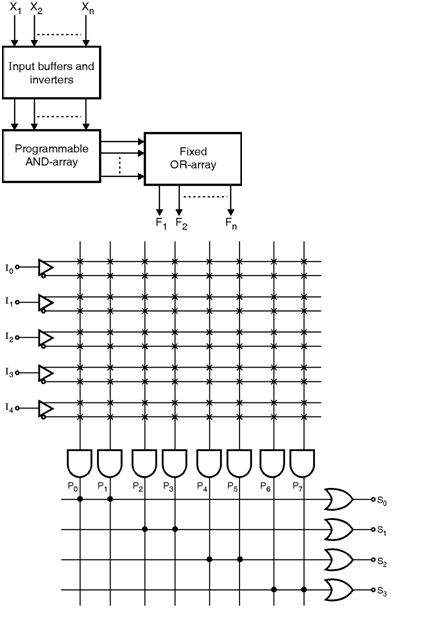
\includegraphics[width=\columnwidth]{figures/pal_2.png}
        \captionof{figure}{PAL architecture with 5 inputs, 8 programmable AND gates and 4 fixed OR gates}
        \label{fig:pal_2}
        % https://www.electronics-tutorial.net/Programmable-Logic-Device-Architectures/Programmable-Logic-Devices/Programmable-Array-Logic-PAL/
        % https://www.naukri.com/code360/library/difference-between-pla-and-pal 
    }

    \newcolumn

    \textbf{Homogeneous FPGA:} \quad 
    The mid-1980s saw the introduction of homogeneous FPGAs, which were built as a grid of CLBs. 
    Rather than using a central programmable switch matrix as in CPLDs, FPGAs adopted an island style architecture in which each CLB is surrounded on all sides by programmable routing resources, as shown in Figure \ref{fig:fpga}. 
    The first commercially viable FPGA, produced by Xilinx in 1984, featured 16 CLBs arranged in a 4x4 grid. 
    As FPGA technology advanced, CLBs were redesigned to use lookup tables (LUTs) instead of PAL arrays for greater logic density. 
    The capacity of an FPGA was often measured by how many logical elements or CLBs it offered, which grew from hundreds to thousands and now to hundreds of thousands of CLBs.
    \\ 

    {
        \centering
        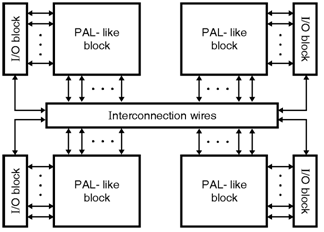
\includegraphics[width=0.8\columnwidth]{figures/cpld.png}
        \captionof{figure}{CPLD architecture with 4 CLBs (PAL-like blocks)}
        \label{fig:cpld}
        % https://www.electronics-tutorial.net/Programmable-Logic-Device-Architectures/CPLD/Complex-Programmable-Logic-Device-CPLDs/
    }
    {
        \centering
        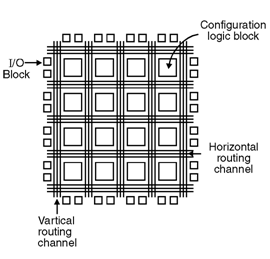
\includegraphics[width=\columnwidth]{figures/homogenous_fpga.png}
        \captionof{figure}{A homogeneous island-style FPGA architecture with 16 CLBs in a grid.}
        \label{fig:fpga}
        % https://www.electronics-tutorial.net/Programmable-Logic-Device-Architectures/FPGA/Field-programmable-gate-array-FPGA/
    }

    \newpage

    {
        \centering
        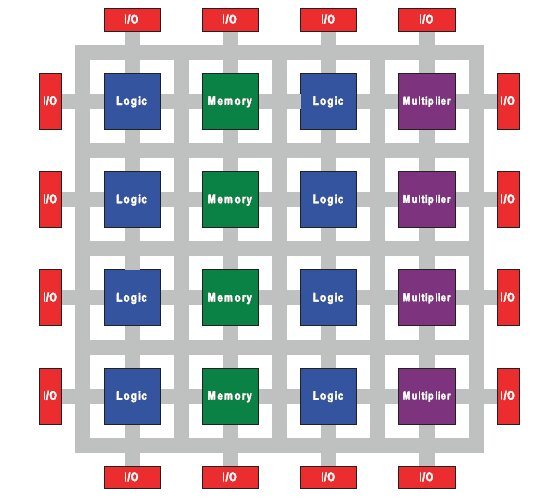
\includegraphics[width=\columnwidth]{figures/heterogenous_fpga_3.jpg}
        \captionof{figure}{A heterogeneous island-style FPGA with a mix of CLBs and macrocells.}
        \label{fig:fpga}
        % https://www.electronics-tutorial.net/Programmable-Logic-Device-Architectures/FPGA/Field-programmable-gate-array-FPGA/
    }
    \vspace{0.5cm}

    \textbf{Heterogenous FPGA:} \quad 
    This brings us to modern day FPGA architectures. 
    To meet the needs of increasingly complex designs, FPGA vendors introduced heterogeneous FPGAs. 
    In these devices, hard macros such as Block RAM (BRAM) and Digital Signal Processing (DSP) slices are integrated into the programmable logic fabric along with CLBs, like shown in Figure \ref{fig:fpga}. 
    This design enables the direct instantiation of common subsystems like memories and multipliers, without having to recreate them from scratch using CLBs. 
    Major vendors such as Xilinx and Altera now employ heterogeneous island-style architectures in their devices. 
    As designs become increasingly large and complex, FPGAs meet the demand by becoming increasingly heterogenous, incorporating a wider variety of hard macros into the fabric. 


\section{Xilinx 7-Series Architecture}
    \label{sec:7_series}
    The Xilinx 7-Series devices, first introduced in 2010, follow a heterogeneous island-style architecture as discussed previously. 
    Although the 7-Series was later superseded in 2013 by the UltraScale architecture, the 7-Series remains highly relevant due to its accessibility, wide availability, and compatibility with open-source tooling. 
    Representative sub-families include Artix-7, Kintex-7, Virtex-7, and Zynq-7000, each designed with different performance and cost trade-offs but all follow the core 7-Series architecture.


    Figure~\ref{fig:hierarchy_4} illustrates a high-level view of the hierarchical organization of a 7-Series FPGA. 
    At its lowest level, the device consists of a large array of atomic components called \emph{Basic Elements of Logic}~(\textbf{BELs}). 
    These BELs encompass look-up tables (\textbf{LUTs}), flip-flops (\textbf{FFs}), block RAMs (\textbf{BRAMs}), DSP slices (\textbf{DSPs}), and the configurable interconnect fabric. 
    They constitute the fundamental building blocks for implementing digital circuits on the FPGA.
    Note how the Tile arrangement is columnar, where each column will have only one Tile type. 

    To manage this complexity, Xilinx organizes these BELs into incrementally abstract structures. 
    First, \textbf{BELs} are grouped into \textbf{Sites}. 
    Each Site is embedded into a \textbf{Tile}, and Tiles are further arranged into \textbf{Clock Regions}. 
    In some high-density devices, multiple Clock Regions may be consolidated into one or more \textbf{Super Logic Regions}~(SLRs). 
    However, for the scope of this paper, we focus on Xilinx 7-Series devices with only a single SLR.

    \end{multicols}
    {
        \centering
        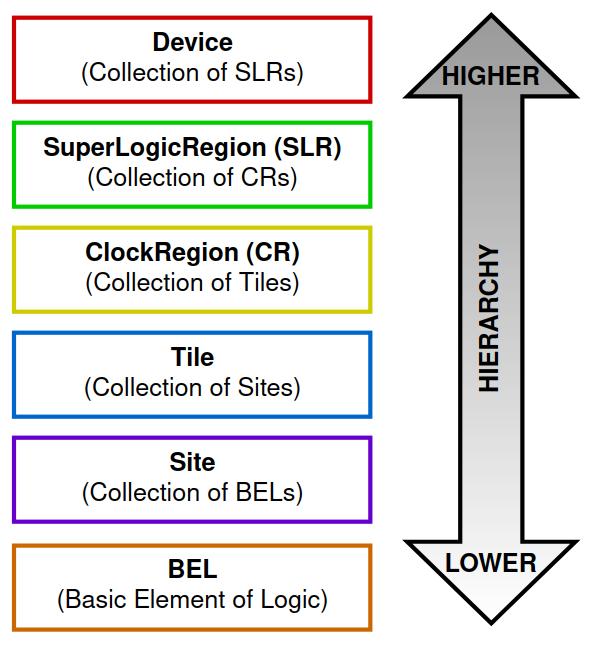
\includegraphics[valign=c, width=0.3\columnwidth]{figures/hierarchy_5.png}
        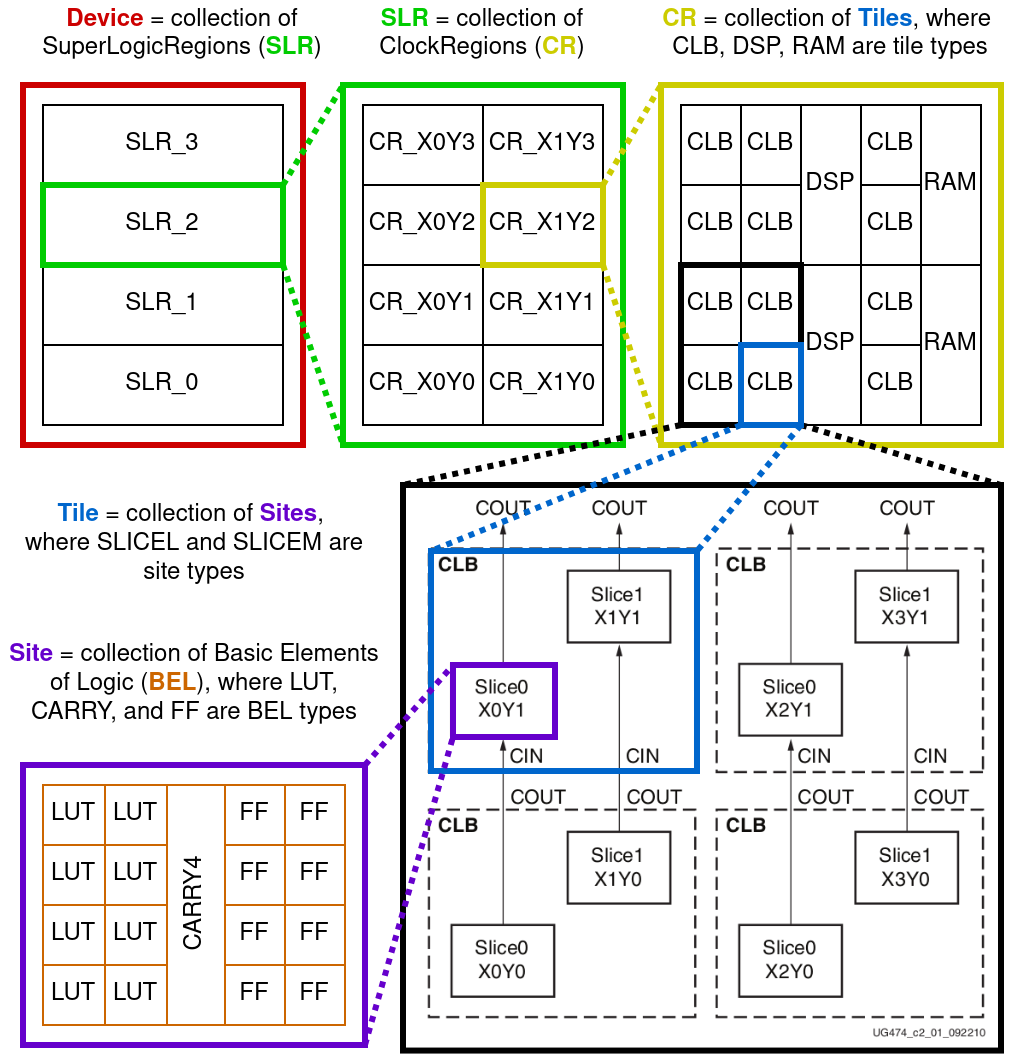
\includegraphics[valign=c, width=0.6\columnwidth]{figures/hierarchy_4.png}
        \captionof{figure}{Architecture Hierarchy of a Xilinx FPGA}
        \label{fig:hierarchy_4}
    }
    \vfill
    \begin{multicols}{2}

    \newpage
    \subsection{CLB SLICEs}

    In the 7-Series architecture, the term \emph{CLB} (Configurable Logic Block) refers to a \emph{CLB Tile} that contains two \emph{SLICE} Sites. 
    Xilinx offers two variants of SLICE Sites: \textbf{SLICEL} and \textbf{SLICEM}.
    \begin{itemize}
        \item Each \textbf{SLICEL} has a set of BELs including eight LUTs, eight FFs, and one   \emph{CARRY4} adder. The LUT BELs in a SLICEL can only host LUT Cells. 
        \item The \textbf{SLICEM} includes all the features of a SLICEL but its LUT BELs can host both LUT Cells, which are asynchronous ROM elements, or RAM32M Cells, which are synchronous 32-deep RAM elements. These cells are also referred to as \emph{Distributed RAM} in the Xilinx documentation.
        These cells can offer an alternative to the larger, more dedicated 18K-36K RAMB18E1 cells when RAM resources are highly utilized. 
    \end{itemize}
    In a typical 7-Series device, approximately 75\% of the SLICE Sites are SLICELs and 25\% are SLICEMs. 
    A single CLB Tile can therefore host either two SLICELs or one SLICEL and one SLICEM.
    For simplicity, however, we will only consider SLICELs for general logic and use the dedicated RAMB18E1 cells to implement RAM elements. 

    The BELs in these SLICEs facilitate the bulk of the general programmability of the FPGA fabric. 
    We will explain in detail the motivation and function of these BELs. 


    \textbf{LUTs} \quad
        Combinational logic is universal to all HDL designs. 
        As the their name suggests, Look‑Up Tables (LUTs) facilitate combinational logic by acting as tiny asynchronously‑accessed ROMs whose contents are fixed when the FPGA is programmed.  
        For any boolean function, the synthesizer precalculates the output to every possible input combination and stores the resulting truth table into a LUT's static memory. 
        The inputs are then essentially treated as an address space that maps to a data value space in an asynchronous ROM. 
        No explicit logic gates like NAND or XNOR are synthesized, contrary to what newcomers might expect from a "Field Programmable Gate Array". 

        {
            \centering
            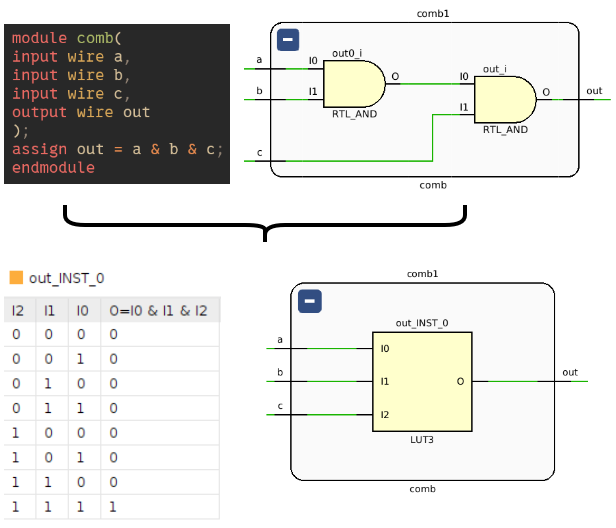
\includegraphics[width=\columnwidth]{figures/lut_synthesis.png}
            \captionof{figure}{LUT synthesis from user design}
            \label{fig:lut_synthesis}
        }
        \vspace{1.0cm}

        In the 7‑Series devices, one LUT can facilitate any 6-input boolean function, or two 5-input functions, as long as they share the same input signals.  
        The LUT can also host two independent boolean functions of up to 3 inputs each, even when the inputs are not shared.  
        Functions requiring more than six unique inputs are decomposed across multiple cascaded LUTs.
        Figure \ref{fig:lut_synthesis} shows an example of where a LUT is typically synthesized in a design entry. 


    \textbf{FFs} \quad
        FFs are synthesized to facilitate synchronous event-driven signal assignment. 
        For most Verilog users, this generally means signal assignments wrapped in \texttt{always @(posedge clk)} statements. 
        Figure \ref{fig:ff_synthesis} shows an example of where a flip flop (FF) is typically synthesized. 
        The cell primitive \textbf{FDRE} is a type of FF and belongs to a family of D Flip Flops (DFFs) with Clock Enable (CE). 
        \begin{itemize}
            \item FDCE - DFF with CE and Asynchronous Clear
            \item FDPE - DFF with CE and Asynchronous Preset
            \item FDSE - DFF with CE and Synchronous Set
            \item \textbf{FDRE} - DFF with CE and Synchronous Reset
        \end{itemize}
        In a typical HDL design, the vast majority of FFs will be synthesized as FDREs with the occasional FDSE, as it is generally good practice to keep FPGA designs synchronous. 
        A FF BEL may also host a LATCH Cell, however, since they are generally bad practice in FPGA design, we will not consider latches in this paper. 

        {
            \centering
            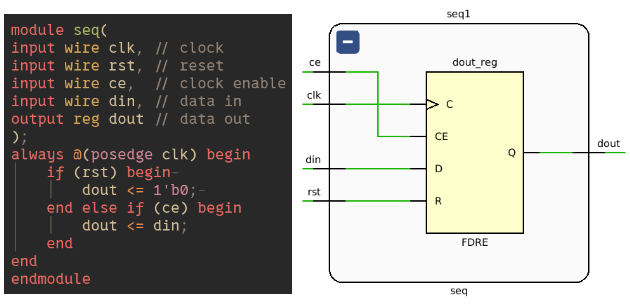
\includegraphics[width=\columnwidth]{figures/ff_synthesis.png}
            \captionof{figure}{FF synthesis from user design}
            \label{fig:ff_synthesis}
        }
        \vspace{1.0cm}

        Up to eight (8) FFs can be placed within the same SLICE, but only if they all share a common Clock-Enable (CE) net and a common Set-Reset (SR) net.
        This is because the SLICE has only one CE pin and one SR pin to interface with general routing. 
        The CE and SR signals from these pins are broadcast intra-Site to all FFs within. 


    \newpage
    \textbf{LUT-FF Pairs} \quad
        FPGA designs are very often modelled as a collection of Finite State Machines (FSM) like shown in Figure \ref{fig:fsm}.
        Many times a design will also use pipelining, either to model signal buffers or shift registers, or to split up large combinational logic blocks into time slices to meet timing constraints. 
        These common design structures result in many consecutive sections of combinational logic feeding into a vector of registers. 
        The synthesizer naturally synthesizes these structures as consecutive pairs of LUTs feeding into FFs as shown in Figure \ref{fig:pipelining}. 
        Figure \ref{fig:lut_ff_pair} shows an example of a synthesized LUT-FF Pair. 

        Shown in Figure \ref{fig:intersite_intrasite} are two possible placements for a LUT-FF Pair on the physical device. 
        On the right, the cells are placed across different Sites, thus the only way to route the net between the cells is through general inter-site routing. 
        On the bottom left, the cells are placed within the same Site in the same lane, taking advantage of the intra-site routing without burdening the general router with additional inter-site routing. 
        This is an important consideration to make while minimizing wirelength during placement. 


        \vspace{1.0cm}
        {
            \centering
            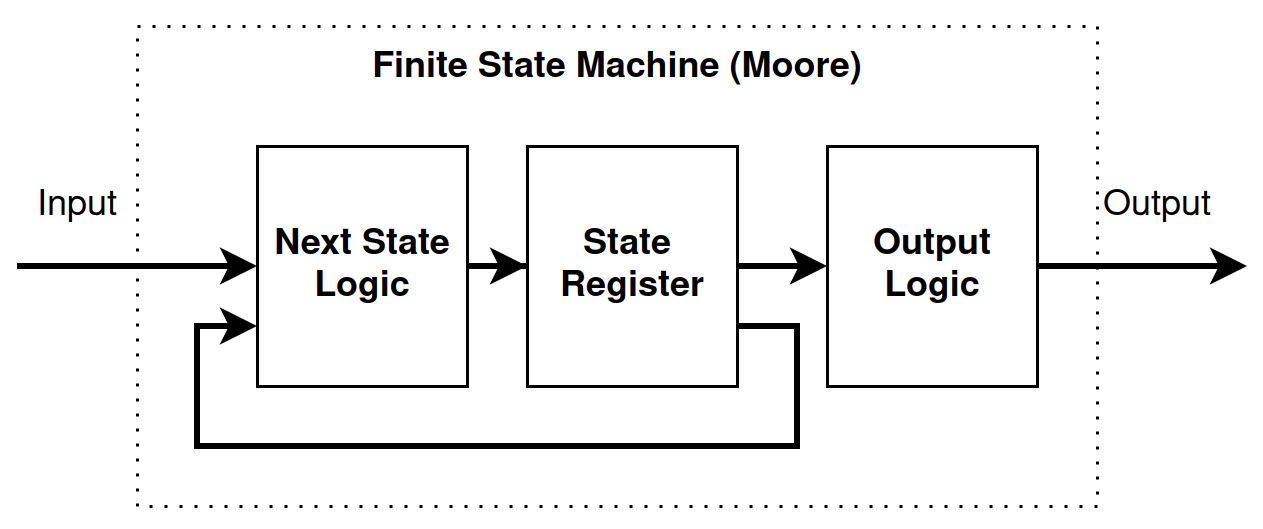
\includegraphics[width=\columnwidth]{figures/fsm.png}
            \captionof{figure}{Finite state machine (Moore)}
            \label{fig:fsm}
        }
        \vspace{1.0cm}

        {
            \centering
            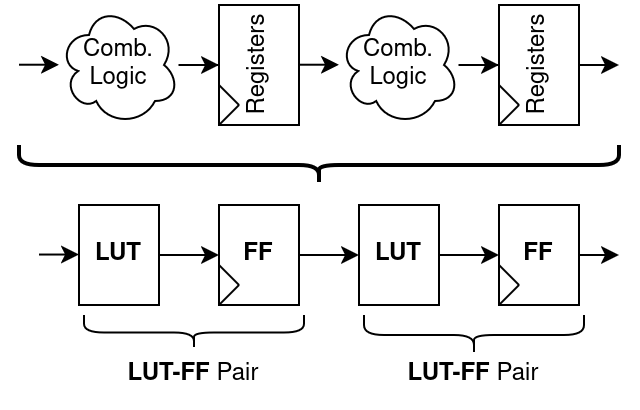
\includegraphics[width=0.9\columnwidth]{figures/pipelining.png}
            \captionof{figure}{Pipelining synthesized as consecutive LUT-FF pairs}
            \label{fig:pipelining}
        }

        \vfill
        .
        \newcolumn

        {
            \centering
            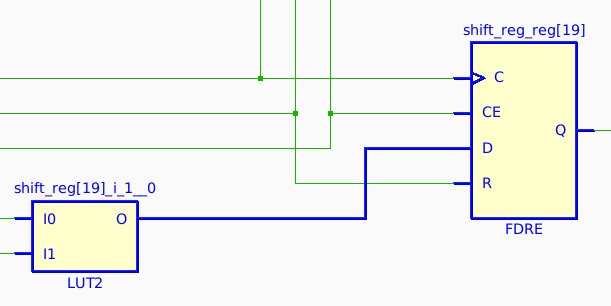
\includegraphics[width=0.9\columnwidth]{figures/lut_ff_pair.png}
            \captionof{figure}{A synthesized LUT-FF Pair}
            \label{fig:lut_ff_pair}
        }
        \vspace{1.0cm}

        {
            \centering
            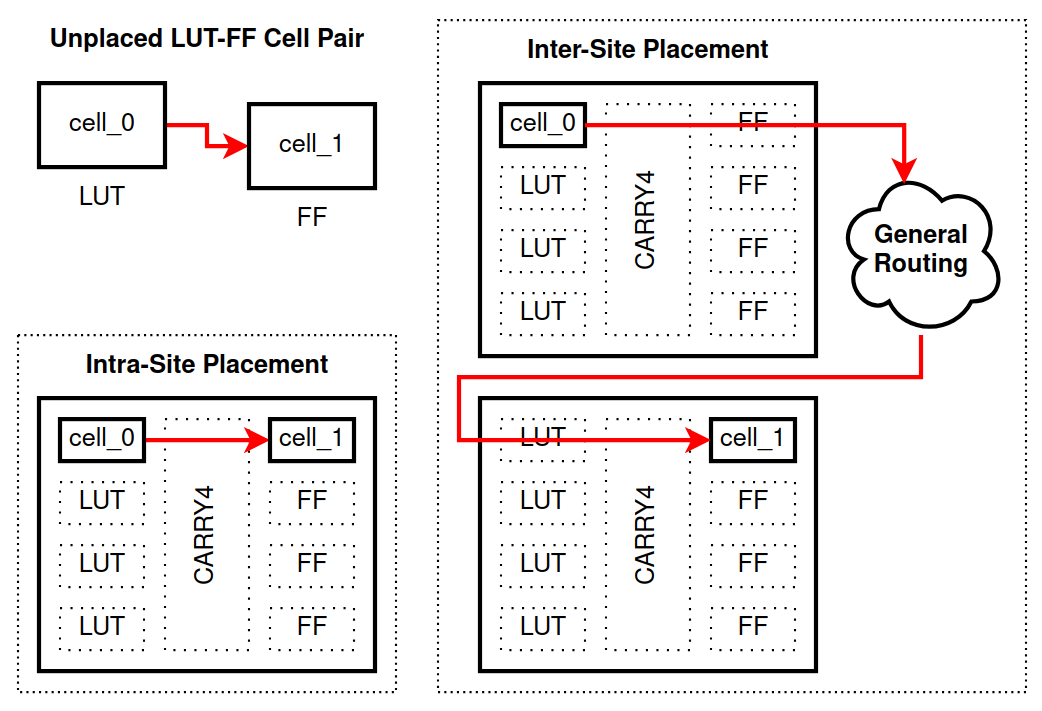
\includegraphics[width=\columnwidth]{figures/intersite_intrasite_2.png}
            \captionof{figure}{Intrasite vs Intersite LUT-FF Placement}
            \label{fig:intersite_intrasite}
        }


    \newpage
    \textbf{CARRY} \quad
        An FPGA design will also typically implement many adders, counters, subtractors, or comparators, all of which are based on binary addition. 
        They are so ubiquitous that every that in the 7-Series architecture, every SLICE features a \emph{CARRY4} BEL -- a 4-bit carry-lookahead (CLA) adder, a much better alternative to synthesizing adders via LUTs. 

    \textbf{CARRY Chains} \quad
        These CARRY4 blocks can be chained across SLICEs to implement wide adders efficiently. 
        The CARRY4 BELs \emph{must} be chained vertically consecutively across SLICEs as the Carry-In (CI) and Carry-Out (CO) pins can only be routed this way. 
        A CARRY4 cell may also directly connect to LUTs and FFs, and should be placed in the same Site whenever possible to minimize wirelength. 
        Shown in figure \ref{fig:carry_cell_group} shows how a CARRY4 chain and associated LUTs and FFs can be placed across SLICEs. 


        {
            \centering
            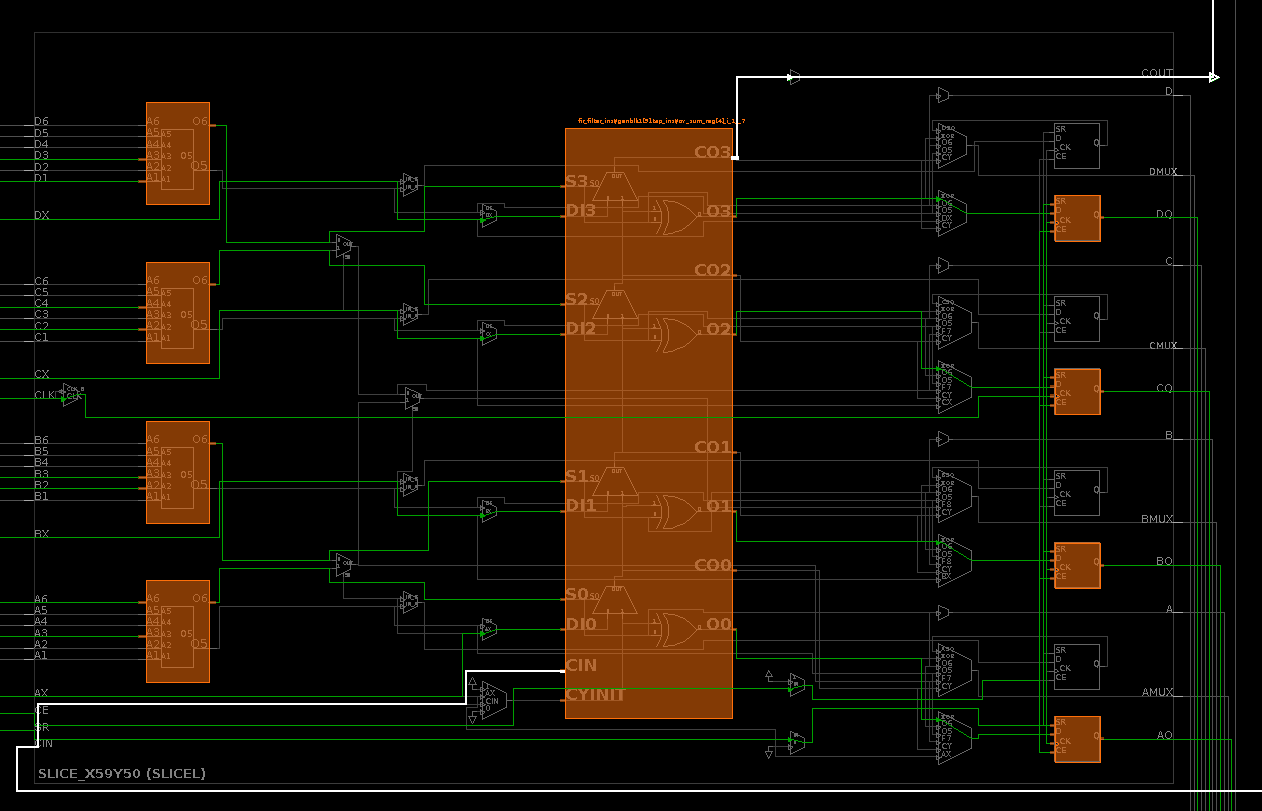
\includegraphics[width=\columnwidth]{figures/carry_cell_group.png}
            \captionof{figure}{A SLICEL with a CARRY4 cell, 4 LUT cells, and 4 FF cells placed inside as shown in the Vivado device viewer}
            \label{fig:carry_cell_group}
        }

        {
            \centering
            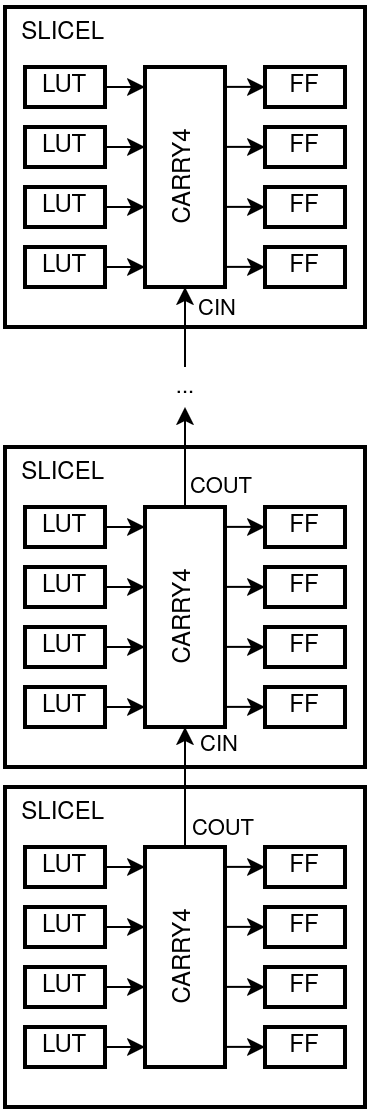
\includegraphics[valign=c, width=4.0cm]{figures/carry_chain_placement.png}
            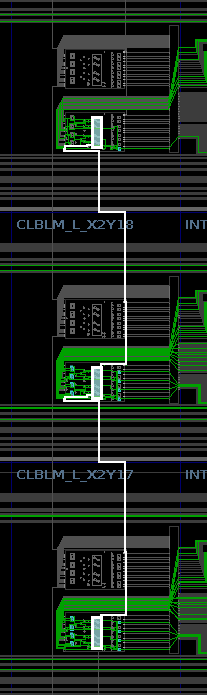
\includegraphics[valign=c, width=4.0cm]{figures/carry_chain_routes_3.png}
            \captionof{figure}{
                A CARRY4 chain of size 3 placed across 3 SLICEs.
                \textbf{Left:} Simplified view, \textbf{Right:} As shown in the Vivado device viewer.
            }
            \label{fig:carry_cell_group}
        }

        \end{multicols}
        % \vfill
        {
            \centering
            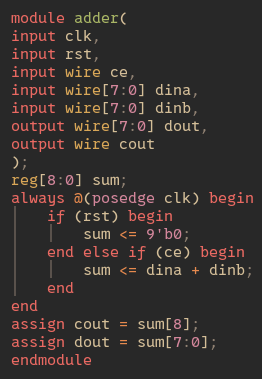
\includegraphics[valign=c, width=3.0cm]{figures/adder_synthesis.png}
            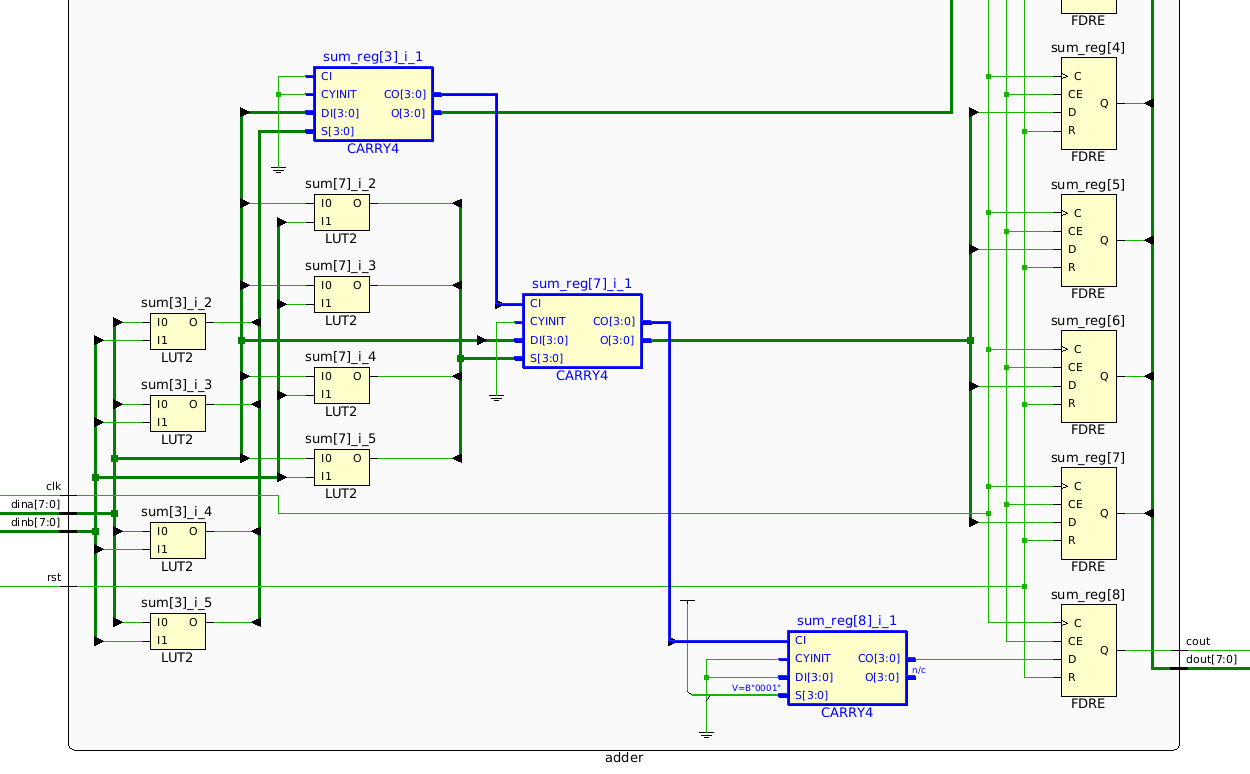
\includegraphics[valign=c, width=14.0cm]{figures/carry_chain_edif_3.png}
            \captionof{figure}{A synthesized carry chain of size 3 as shown in the Vivado netlist viewer}
            \label{fig:carry_chain_edif}
        }
        \begin{multicols}{2}
        \vspace{1.0cm}
        .

    \newpage
    \subsection{DSP Slices}

    \textbf{DSPs} \quad 
        FPGAs are often used as low latency Digital Signal Processing (DSP) accelerators. 
        Common DSP subsystems like Finite Impulse Response (FIR) filters, Fast Fourier Transform (FFTs), and convolutional neural nets (CNNs) demand fast large scale multiply-accumulate (MAC) capabilities. 
        The 7-Series arhictecture integrates DSP BELs into the logic fabric called DSP48E1 that can facilitate MAC efficiently. 
        The architecture hierarchy for DSPs is simple compared to CLBs and SLICEs. 
        A DSP48E1 Tile contains two DSP48E1 Sites, each containing one DSP48E1 BEL, which can host a DSP48E1 Cell. 

        {
            \centering
            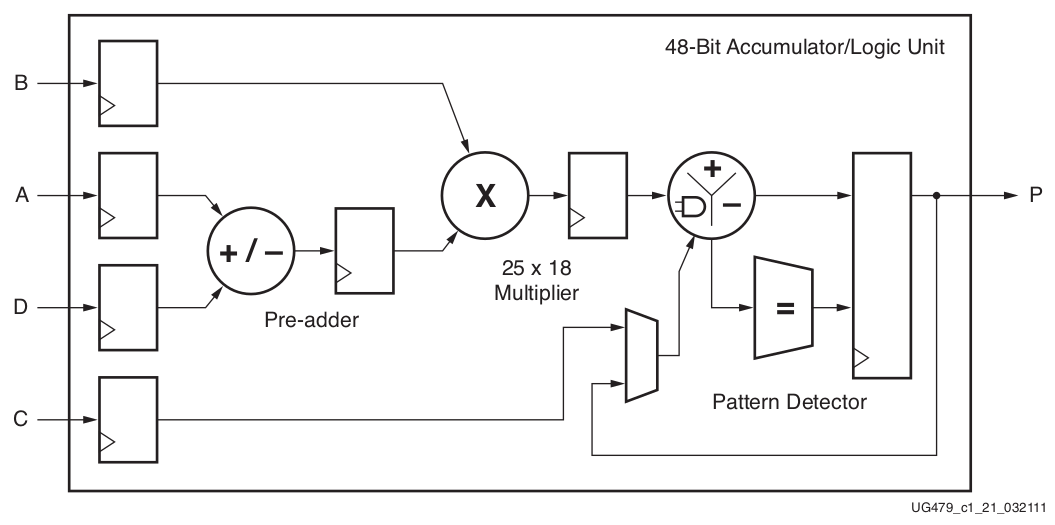
\includegraphics[width=\columnwidth]{figures/dsp_diagram.png}
            \captionof{figure}{
                Basic DSP48E1 Slice Functionality
            }
            \label{dsp_diagram}
        }
        \vspace{0.5cm}

    \textbf{DSP Cascades} \quad 
        Higher level DSP functions are supported by cascading DSP48E1 slices in a DSP48E1 column.
        Much like CARRY4 chains, DSP48E1 cascades must necessarily be placed vertically consecutively across DSP48E1 Sites. 
        They are connected by three busses: ACOUT to ACIN, BCOUT to BCIN, PCOUT to PCIN.
        These signal busses run directly between the vertical DSP48E1 slices without burdening the general routing resources. 
        The ability to cascade this way provides a high-performance and low-power implementation of DSP filter functions. 

        \vspace{1.0cm}
        {
            \centering
            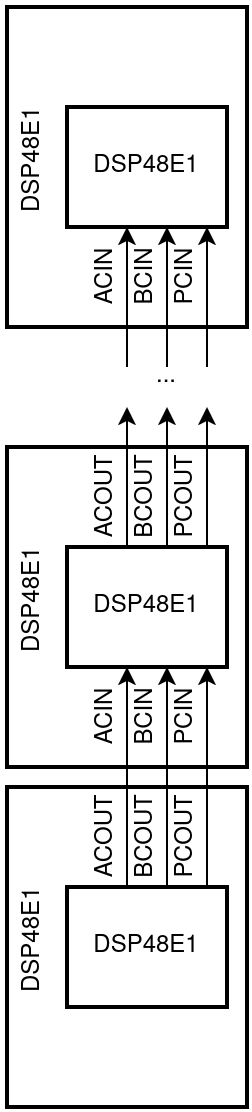
\includegraphics[valign=c, width=2.5cm]{figures/dsp_cascade_placement.png}
            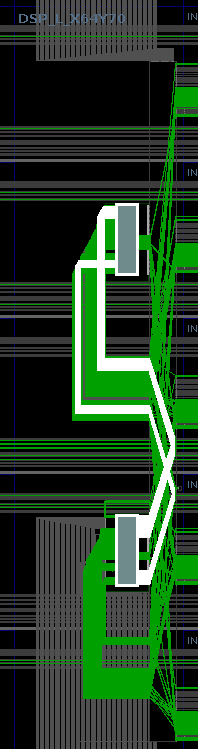
\includegraphics[valign=c, width=3.0cm]{figures/dsp_cascade_routed.png}
            \captionof{figure}{
                A DSP48E1 cascade of size 2 placed across 2 DSP48E1 Sites.
                \textbf{Left:} Simplified view, \textbf{Right:} As shown in the Vivado device viewer.
            }
        }

        \end{multicols}
        {
            \centering
            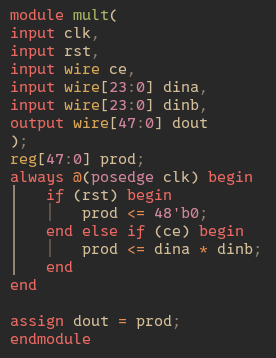
\includegraphics[valign=c, width=4.0cm]{figures/mult_synthesis.png}
            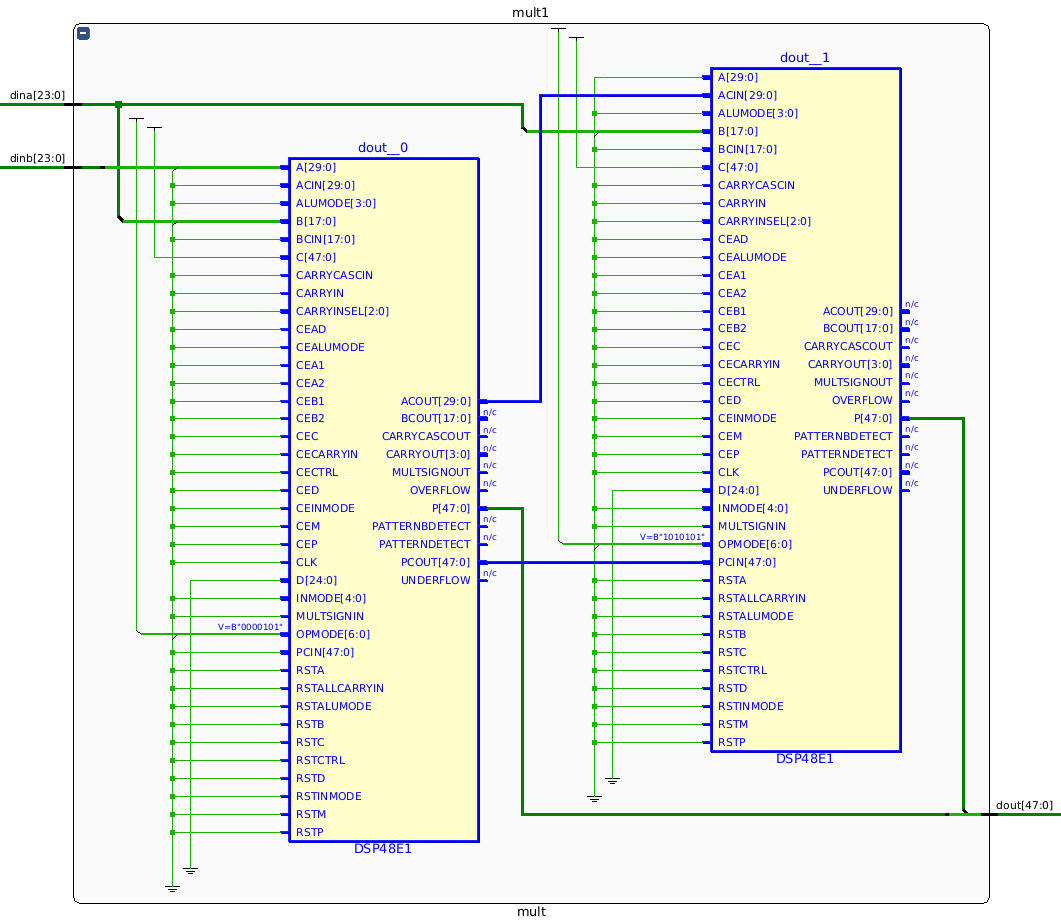
\includegraphics[valign=c, width=13.0cm]{figures/dsp_synthesis.png}
            \captionof{figure}{
                Simple multiplier synthesis from user design.
            }
            \label{mult_synthesis}
        }
        \begin{multicols}{2}


    \newpage

    \subsection{Block RAM}
        In addition to SLICEs and DSPs, the 7-Series also offers dedicated Block Random Access Memory (BRAM) BELs. 
        These BRAMs come in two variants: \textbf{RAMB18E1} and \textbf{RAMB36E1}. 
        \begin{itemize}
            \item \textbf{RAMB18E1} - 
            Has a capacity of 18 Kilobits. 
            It can be configured as single port RAM with dimensions ranging between (1-bit wide by 16K deep) to (18-bit wide by 1024 deep). 
            It can also be configured as a (36-bit wide by 512 deep) true simple dual port RAM. 
            \item \textbf{RAMB36E1} - 
            Has a capacity of 36 Kilobits. 
            It can be configured as single port RAM with dimensions ranging between (1-bit wide by 32K deep) to (36-bit wide by 1024 deep). 
            It can also be configured as a (72-bit wide by 512 deep) simple dual port RAM. 
        \end{itemize}

        For readability, we will abbreviate RAMB18E1 as \textbf{RAM18} and RAMB36E1 as \textbf{RAM36}.
        One BRAM Tile contains one RAM36 Site and two RAM18 Sites. 
        The RAM36 Site contains one RAM36 BEL while the RAM18 Site contains one RAM18 BEL.
        The RAM18 BEL can host one RAM18 Cell, while the RAM36 BEL can host either one RAM36 Cell or two RAM18 Cells. 

        Like DSP cascades, BRAMs may also be cascaded together in a column to implement large memories efficiently, with some intermediate signals between them routed intra-Tile without burdening the general routing. 
        However, unlike DSPs, large memories decomposed amongst multiple BRAMs can also be routed together through general routing. 
        Furthermore, in most design scenarios, large memories will not utilize the intra-Tile signals. 
        
        For simplicity we will not constrain large BRAMs to be cascaded together in consecutive vertical Tiles. 
        We can essentially treat RAMB18E1 and RAMB36E1 Cells as loose, minimally constrained single cells, in contrast to the highly constrained DSP cascades and CARRY chains.

        {
            \centering
            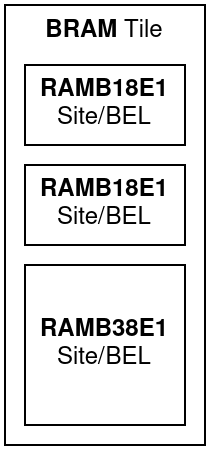
\includegraphics[valign=c, width=3.0cm]{figures/bram.png}
            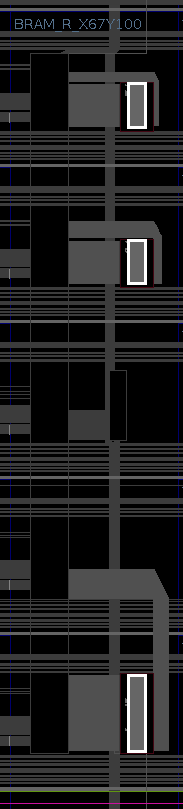
\includegraphics[valign=c, width=2.0cm]{figures/bram_tile.png}
            \captionof{figure}{
                A BRAM Tile containing two RAMB18E1 Sites and one RAMB36E1 Site.
                \textbf{Left:} simplified view. \textbf{Right:} as seen in the device viewer, BELs highlighted in white. 
            }
            \label{fig:bram_tile}
        }

        {
            \centering
            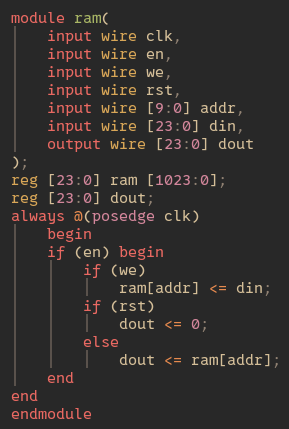
\includegraphics[valign=c, width=4.0cm]{figures/bram_synthesis.png}
            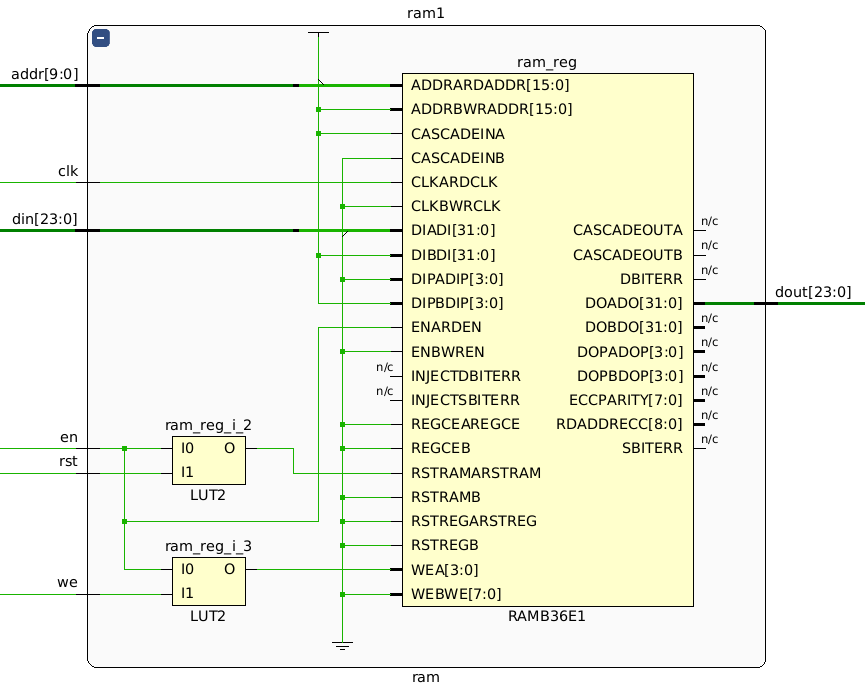
\includegraphics[valign=c, width=\columnwidth]{figures/bram_edif.png}
            \captionof{figure}{
                An example of BRAM synthesis (via inference)
            }
            \label{fig:bram_synthesis}
        }

    \subsection{Further Documentation}

    For more in-depth details about 7-Series FPGAs, refer to the official Xilinx user guides such as:
    \begin{itemize}
        \item \emph{7 Series FPGAs Overview} (UG476)
        \item \emph{7 Series FPGA Configurable Logic Block} (UG474)
        \item \emph{7 Series Memory Resources} (UG473)
        \item \emph{7 Series DSP48E1 Slice} (UG479)
    \end{itemize}

    This architectural context provides the necessary background for understanding how a placement algorithm should account for resource constraints and optimize performance in modern FPGA designs.


\newpage
\section{FPGA Design Flow and Toolchain}
    \label{sec:fpga_flow_toolchain}

    Modern FPGA designs require a sophisticated toolchain to bridge the gap between high-level hardware descriptions and the final bitstream used to configure the FPGA. 
    Figure~\ref{fig:design_flow} illustrates a representative process that converts an abstract Hardware Description Language (HDL) design into a verified configuration file for a target device.

    {
        \centering
        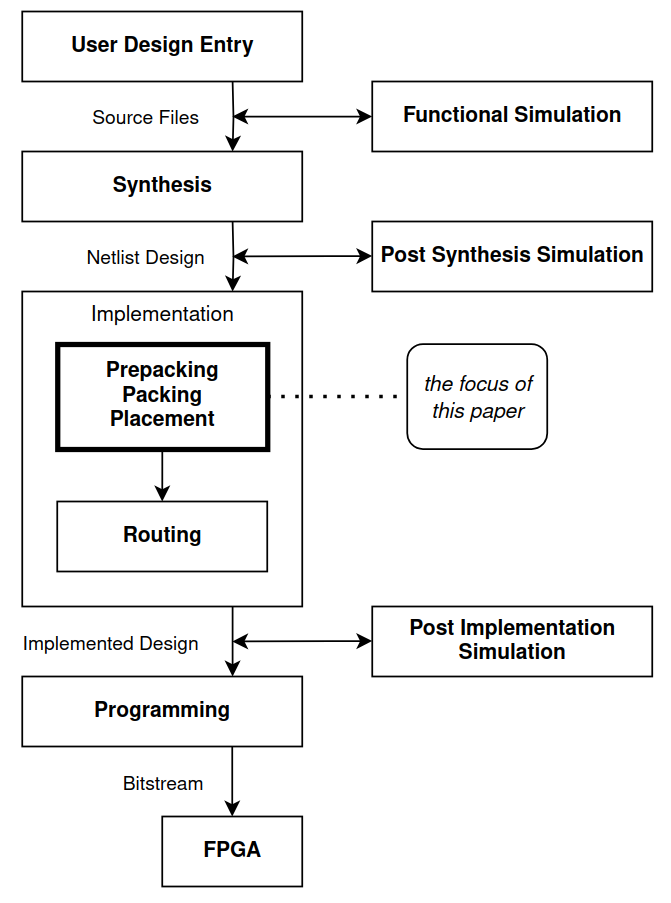
\includegraphics[width=0.9\columnwidth]{figures/design_flow.png}
        \captionof{figure}{A typical FPGA design and verification workflow.}
        \label{fig:design_flow}
    }

    \begin{enumerate}
        \item \textbf{Design Entry:} 
            An engineer describes the intended functionality of the digital system using a hardware description language (HDL) such as Verilog or VHDL. 
            During this phase, the coding style can vary (behavioral, structural, dataflow, etc.), but it always aims to capture high-level behavior rather than device-specific details.

        \item \textbf{Synthesis:} 
            The synthesis tool parses the HDL source, performs logical optimizations, and maps the design onto primitive cells that suit the target FPGA technology. 
            The output is typically a \emph{structural} netlist (e.g., EDIF or structural Verilog) which details how the design’s logic is broken down into LUTs, FFs, and other vendor-specific cells.

        \item \textbf{Placement and Routing (Implementation):} 
            In \emph{placement}, each logical cell from the synthesized netlist is assigned to a physical location on the FPGA fabric. 
            For instance, LUTs and FFs go into specific \emph{BELs} within the device’s CLB sites, and specialized cells such as DSPs and Block RAMs must be placed in their corresponding tile types. 
            Next, \emph{routing} determines how signals are physically wired through the FPGA’s configurable interconnect network. 
            Modern tools often interleave these steps (e.g., fluid-placement routing or routing-aware placement) to better meet timing and area objectives.

        \item \textbf{Bitstream Generation:} 
            After a design is fully placed, routed, and timing-closed, the toolchain produces a final \emph{bitstream} that sets the configuration of every programmable element in the FPGA. 
            This bitstream can then be loaded onto the device, either through vendor software or via a custom programming interface.

        \item \textbf{Verification:} 
            In parallel to the design flow, simulations and testbenches validate correctness of the user's design at multiple abstraction levels. 
            Engineers may begin with behavioral simulations, then progress to post-synthesis simulations, and finally to post-implementation simulations that incorporate estimated routing delays. 
            With each higher level of fidelity, computational requirements grow significantly due to increasing complexity and the need to analyze more variables over time. 
            Ensuring correct functionality and meeting timing closure at the post-implementation stage is crucial before deploying the design to hardware. 
            Given the importance of thorough verification, many established companies dedicate one verification engineer for every design engineer.

    \end{enumerate}

    This workflow underscores the critical role of \textbf{placement} in bridging the netlist to a physical realization. 
    An efficient placement algorithm can drastically reduce compile times and improve design performance, enabling broader adoption of FPGAs in application spaces that require fast design iteration.


\section{RapidWright API}
    \label{sec:rapidwright_api}

    \textbf{RapidWright} is an open-source Java framework from AMD/Xilinx that provides direct access to the netlist and device databases used by vendor tools. 
    This framework positions itself as an additional workflow column, allowing users to intercept or replace stages of the standard design flow with custom optimization stages (see Figure~\ref{fig:vivado_dcps}).

    \begin{itemize}
    \item \textbf{Design Checkpoints:} 
        RapidWright leverages \texttt{.dcp} files (design checkpoints) generated at various stages of a Vivado flow. 
        By importing a checkpoint, engineers can manipulate the netlist, placement, or routing externally, then re-export a modified checkpoint for further processing in the Vivado workflow column.

    \item \textbf{Key Packages:} 
        RapidWright revolves around three primary data model packages:
        \begin{enumerate}
        \item \emph{edif} -- Represents the logical netlist in an abstracted EDIF-like structure.
        \item \emph{design} -- Contains data structures for the physical implementation (Cells, Nets, Sites, BELs, etc.).
        \item \emph{device} -- Provides a database of the target FPGA architecture (e.g., Site coordinates, Tile definitions, routing resources).
        \end{enumerate}

    \item \textbf{Interfacing with the Netlist and Device:} 
        An engineer can query the netlist to find specific resources (LUTs, FFs, DSPs, etc.) and then map or move them onto device sites. 
        This level of control over backend resources is necessary for research in custom placement, advanced packing techniques, or experimental routing algorithms.
    \end{itemize}

    {
        \centering
        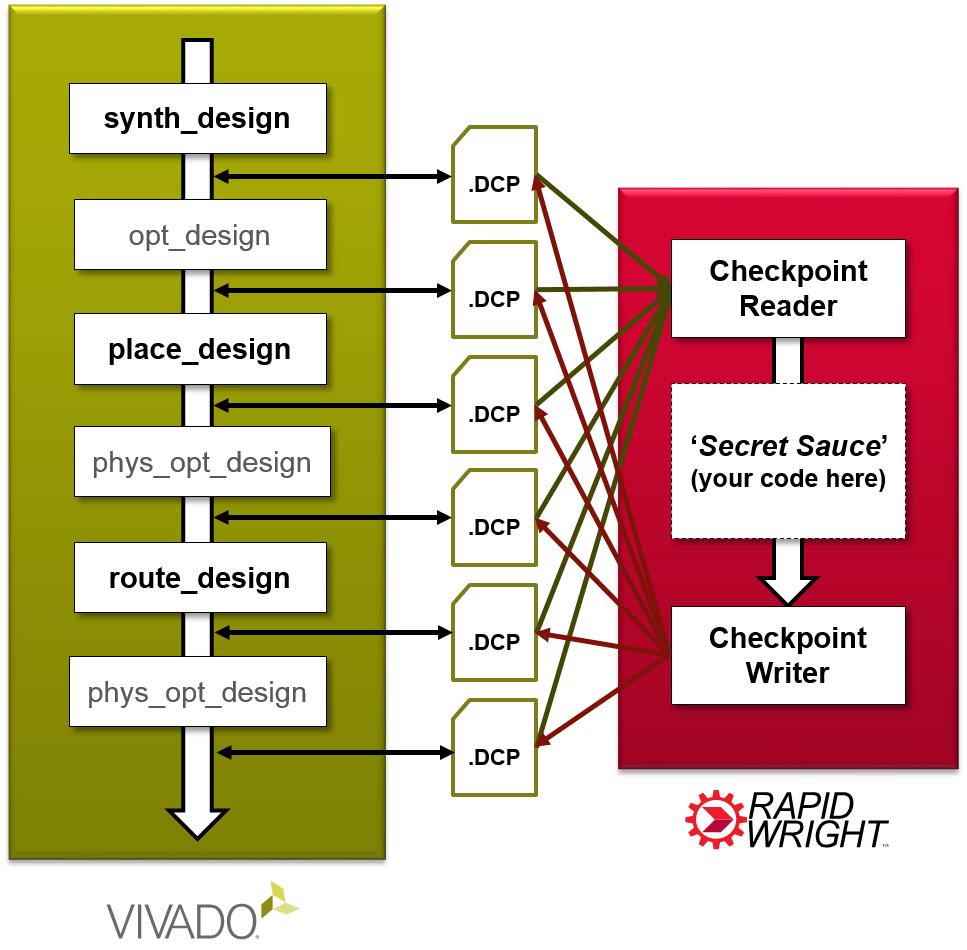
\includegraphics[width=0.8\columnwidth]{figures/vivado_dcps.png}
        \captionof{figure}{RapidWright workflow integrating into the default Vivado design flow.}
        \label{fig:vivado_dcps}
    }

    By exposing these low-level internals, RapidWright allows fine-grained design transformations that go beyond the standard Vivado IDE’s capabilities. 
    Researchers can prototype new EDA strategies without needing to re-implement an entire FPGA backend from scratch, thus accelerating innovation in placement and routing methodologies.

\section{Simulated Annealing}
    \label{sec:simulated_annealing}
    With a basic understanding of FPGA architecture, design placement, and RapidWright, we have all the necessary pieces to implement our SA placer. 
    Here we outline in detail each substage of our implementation: PrePacking, Packing, and Placement. 
    Shown in Figure \ref{fig:edif_design_device} shows an overview of the placement workflow. 

    {
        \centering
        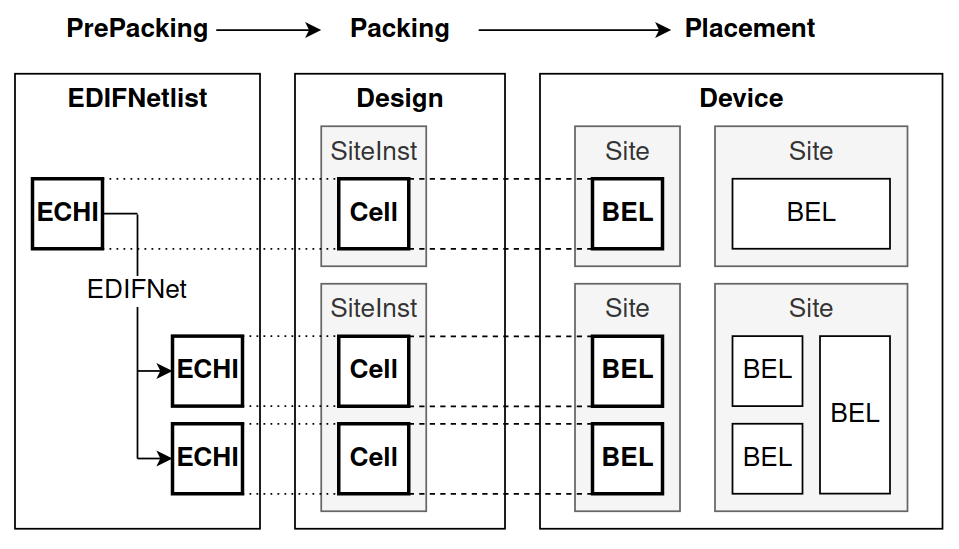
\includegraphics[width=0.9\columnwidth]{figures/edif_design_device.png}
        \captionof{figure}{Our placement workflow}
        \label{fig:edif_design_device}
    }

    \end{multicols}
    {
        \centering
        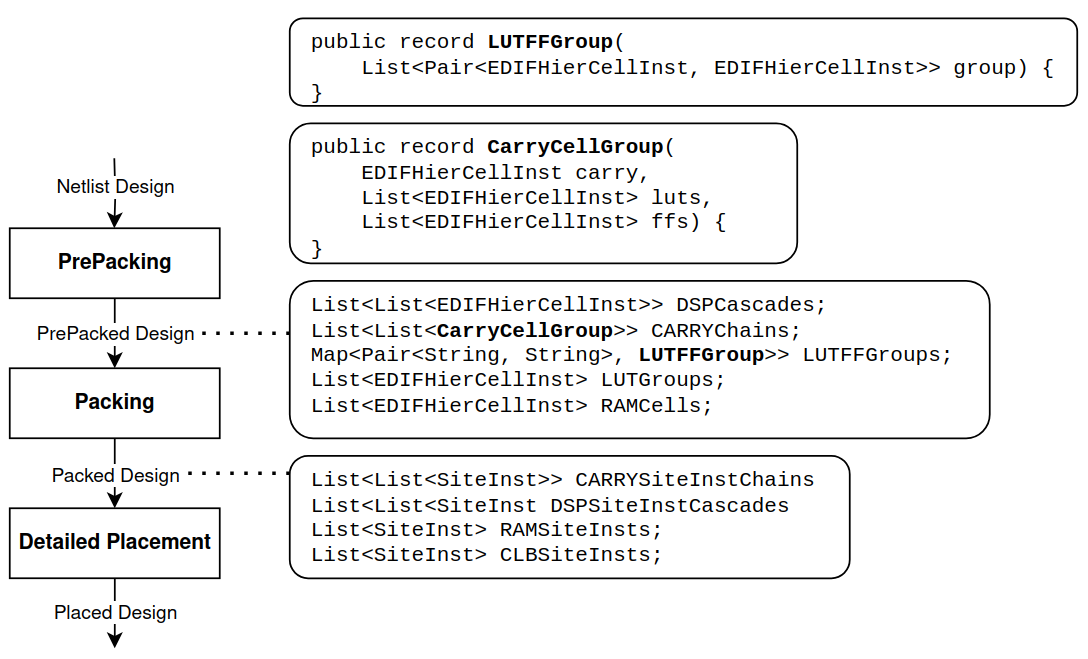
\includegraphics[width=0.8\columnwidth]{figures/substages.png}
        \captionof{figure}{The data classes populated at each substage: PrepackedDesign, PackedDesign, and PlacedDesign.}
        \label{fig:substages}
    }
    \begin{multicols}{2}

    \subsection{Prepacking}
        \label{subsec:prepacking}

        \end{multicols}
        {
            \centering
            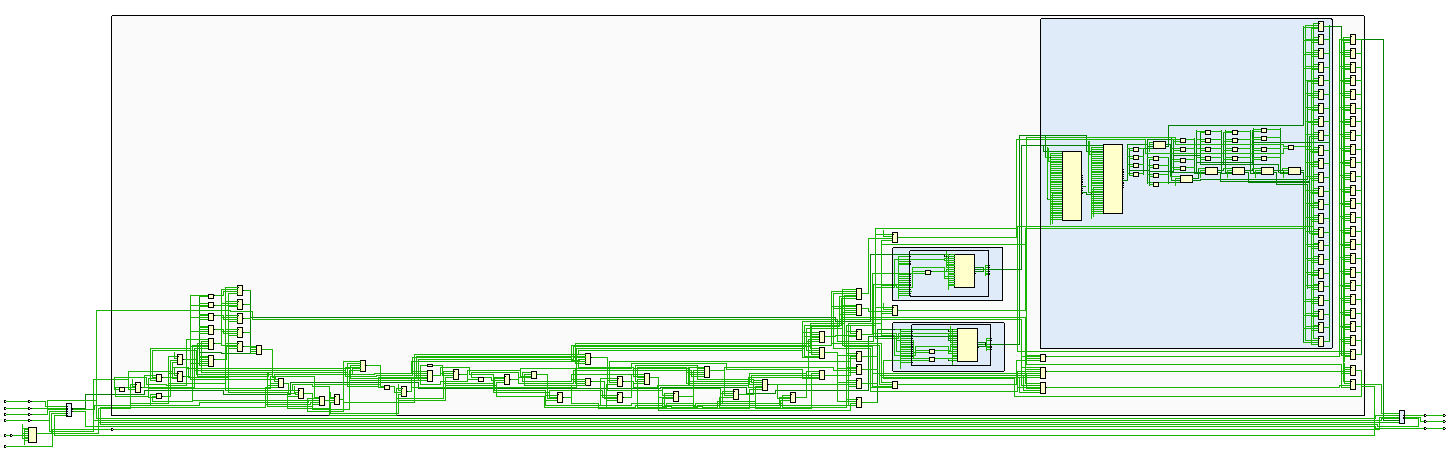
\includegraphics[width=\columnwidth]{figures/raw_edif.png}
            \captionof{figure}{A raw EDIF Netlist with uncountably many cells}
            \label{fig:raw_edif}
        }
        \begin{multicols}{2}

        The first step in our placement flow is \textbf{prepacking}. 
        Recall from the 7-Series architecture that there are certain cell groups that must adhere to certain placements constraints to ensure legality, and by design, to minimize wirelength. 
        CARRY4 chains must necessarily be placed vertically and consecutively across a column of SLICEs in ascending order. 
        Likewise, DSP48E1 cascades must necessarily be placed vertically and consecutively across a column of DSP48E1 Sites in ascending order. 
        A LUT-FF may be placed freely, but should be placed within the same SLICE within the same lane to minimize wirelength.
        A group of LUT-FF pairs may be placed in the same SLICE, with the constraint that the FFs must share the same Clock-Enable (CE) and Set-Reset (SR) nets.
        Clustering LUT-FF pairs like this can reduce the redundancy of having to route the same CE and SR nets to many SLICEs by routing the nets to fewer SLICEs and connecting them to the individual FFs within via intra-Site routing, and at the same time, packing greater logic density over a smaller area of the device. 

        The job of the prepacker is to consolidate functionally related cells from the raw post-synthesis netlist into clusters or groups of clusters that correspond naturally to the physical FPGA architecture. 
        We traverse the netlist to detect and identify LUT-FF pairs, CARRY4 chains, and DSP48E1 cascades. 
        

        LUT-FF pairs, CARRY4 chains, and DSP cascades.
        In this stage, we work solely at the \texttt{edif} level.

        In the context of implementing a custom \emph{Simulated Annealing} (SA) placer, \textbf{prepacking} is the first step in consolidating functionally related cells from the raw post-synthesis netlist into logical clusters that correspond more naturally to the physical FPGA structures. 
        We take a synthesized design checkpoint and open it via RapidWright. 
        We traverse the raw post-synthesis netlist via RapidWright’s \texttt{edif} package to identify LUT-FF Pairs, CARRY4 Chains, DSP Cascades, and remaining single cells.
        We cluster these detected cell structures into their respective \texttt{List}s.


        First, we build the vocabulary of primitive cells by identifying the set of all unique cell types in the EDIF Netlist. 
        We build a \texttt{HashMap}, where the keys are the cell type and the values are \texttt{List}s.


        \textbf{LUT-FF pairs:} \quad
            Most synchronous designs implement finite-state machines or pipelined datapaths, mapping their combinational logic into LUTs directly feeding FFs. 
            Clustering each LUT-FF pair under a single “prepacked object” facilitates usage of dedicated intra-SLICE connections, thereby reducing routing overhead.

        \textbf{CARRY4 chains:} \quad
            Arithmetic operations (adders, counters, comparators) often chain multiple \emph{CARRY4} cells vertically. 
            During prepacking, it is crucial to detect these chains so they remain grouped and placed in physically consecutive and vertical SLICEs for placement legality and optimal performance.

        \textbf{DSP cascades:} \quad
            In designs with large multiply-accumulate structures, DSP48E1 blocks can be used and cascaded along dedicated paths. 
            Identifying such cascades early helps the placer keep them localized, minimizing high-speed interconnect usage.
            Like carry chains, each DSP in a DSP cascades must be placed vertically, in physically consecutive and vertical DSP48E1 Sites.

        \textbf{Loose or Single Cells} \quad
            The remaining cells 
            Various design-specific macros (e.g., BRAM-based FIFOs, shift-register logic) also benefit from being clustered, though these may be addressed in subsequent or more advanced stages.

        This strategy not only reduces the complexity of the placement search space but also helps ensure legality (e.g., shared control signals, shared carry nets). 
        The subsequent \emph{packing} and \emph{placement} steps can then operate on these higher-level groupings with improved efficiency. 

    \subsection{Packing}
        \label{subsec:packing}

    \subsection{Placement}
        \label{subsec:placement}
        Up until now we have only organized the logical \texttt{Cells} into \texttt{SiteInsts}. 
        This is where simulated annealing actually begins. 


\newpage
o
\newpage
%%% OLD

\section{OLD: Simulated Annealing}
    With a basic understanding of FPGA architecture, design placement, and RapidWright, we have all the necessary pieces to implement our SA placer. 
    Here we outline in detail each substage of our implementation: PrePacking, Packing, and Placement. 


    \subsection{PrePacking}
        In the prepacking stage, we traverse the raw post-synthesis EDIF Netlist to identify common recurring Cell patterns. 
        We do this because there are certain desirable cell configurations that should be clustered together to exploit the physical organization of the BELs and Sites of the architecture. 
        Doing so will innately improve wirelength minimization. 
        There are also some cell configurations that must necessarily be placed in certain ways in relation to each other to ensure legality within the architecture constraints. 

        Furthermore, certain cell patterns are specific to certain cell types. 
        Therefore, we must first traverse the entire EDIF netlist and identify all unique cell types and group them together via a {\tt HashMap<String, List<EDIFHierCellInst>>}, where key String is the name cell type and value {\tt List<EDIFHierCellInst>} is the list of cells of that type. 
        The resulting lists in the hashmap are mutually exclusive. 

        Cell types can include {\tt CARRY4}, {\tt LUT1-6}, {\tt FF}, {\tt DSP48E1}, {\tt RAMB18E1}, and others. 
        We specifically look for CARRY4 chains, DSP48E1 cascades, and LUT-FF pairs as these patterns are common to nearly all FPGA designs. 
        We will describe each cell pattern in detail. 

        \subsection{LUT-FF Pairs}
            Very often, engineers model the behavior of a digital system as a collection of Finite State Machines (FSM) as shown in Figure \ref{fig:fsm}. 
            An FSM at its core is a synchronous sequential circuit comprising of a combinational element and a synchronous memory element. 
            In the 7-Series architecture, combinational elements are synthesized as LUTs, where the truth table of the combinational function is mapped onto the LUT's memory. 

            Combinational functions in 7-Series FPGAs are synthesized as Look-Up Tables (LUTs). 
            The FPGA synthesizer maps the combinational element into LUTs and the memory element onto FFs. 

            In the vast majority of HDL designs, LUTs and FFs will be synthesized in pairs, as is the case in Figure \ref{fig:lut_ff_pair}. 
            Shown in Figure \ref{fig:intrasite_intersite} are two possible placements for this cell net. 
            On the right, the cells are placed across different Sites, thus the only way to route the net between the cells is through general inter-site routing. 
            On the bottom left, the cells are placed within the same Site, taking advantage of the intra-site routing and avoiding costly inter-site routing. 

            Identify unique CE-SR net pairs. 
            All FF cells in a Site must share the same CE and SR nets. 


        \subsection{CARRY Chains}


            Figure \ref{fig:carry_cell_edif} shows an example of a CARRY4 cell while figure \ref{fig:carry_chain_edif} shows an example of a CARRY4 chain of size 6. 

            As the name implies, CARRY chains are chains of CARRY cells. 
            % On the Ultrascale architecture, the each CLB contains a CARRY8 BEL, an 8-bit CLA adder, allowing for even greater logic density. 


            (By now Need to have introduced SLICEL / SLICEM Sites and differentiated them from "CLBs", which are referred to as CLBL or CLBM Tiles)
            (rip some figures from the 7-series CLB user guide)

            These CARRY4 cells, if chained together, must be placed vertically across CLBs, as each CLB is connected vertically by a Carry In (CI) to Carry Out (COUT) wire between them. 
            The only way to route the carry net is through this wire, thus why these CLBs must be placed consecutively vertically. 
            This allows the facilitation of fast adders on the device. 

            The CARRY4 
            We identify CARRY4 chains by taking the CARRY4 entry of the HashMap. 
            We follow the below pseudocode 




            Carry chain cells are primitive elements that are provided with a group of LUTs to enable more efficient programmable arithmetic. 
            Primarily it provides dedicated paths for the carry logic of simple arithmetic operations (add, subtract, comparisons, equals, etc). Implementing these arithmetic operations with raw LUTs would results in an inefficient use of resources and performance would suffer. 
            In this way, the CARRY4 cell is like a macrocell. 

            On the device, they must necessarily be arranged consecutively vertically, from bottom to top. 
            Figure \ref{fig:carry_chain_edif} shows an example of a CARRY4 EDIFCell chain in an EDIFNetlist. 
            Notice how there are many different types of cells connected to the CARRY4 Cells. 
            The raw netlist does not tell us the presence of any carry chains or other cell clusterings. 
            We must manually traverse the netlist to identify all of the carry chains by accessing each carry cell, accessing its Ports, accessing the net on the port, accessing all of the other ports on the net, and checking if those ports belong to another carry cell. 
            We continue to traverse the carry chain until the final carry cell is not connected to another carry cell. 
            We must traverse in both directions. 
            After we reach the tail of the current chain, we traverse in the opposite direction (CIN vs COUT) to find the carry chain anchor. 
            We then remove all the cells in this chain from the set of all carry cells. 
            We select the next carry cell in the set of all carry cells and repeat the process, until there are no more remaining carry cells in the set of all carry cells. 


            Shown in figure \ref{fig:carry_cell_edif} 

            To find CARRY chains, we take the CARRY4 group and follow the below pseudocode. 
            Each SLICE Site contains one CARRY4 BEL. 
            Each CLB Tile contains two SLICE Sites. 
            CARRY chains span vertically across multiple SLICE Sites/Tiles. (Show picture) 


        \subsection{DSP Cascades}
            Each DSP Site contains one DSP BEL. 
            Each DSP Tile contains two DSP Sites. 
            DSP chains can span vertically across multiple DSP Sites/Tiles. 


    \subsection{Packing}
        In the packing stage, we take the identified cell clusters and package them into SiteInst Design objects which target the Device Site objects. 
        \subsection{CLB Sites}
            Can support LUT-FF pairs, loose LUTs, loose FFs, CARRY chains. 
            Each SLICE has 8 "lanes" of LUT-FFs. 4 LUT5s and 4 LUT6s. 8 FFs. 
            For SLICEMs, LUT6s can be configured as shallow 32-bit LUTRAMs or "RAMS32". 

    \subsection{Placement: Simulated Annealing} 
        Bookkeeping: keep track of Sites occupied by single SiteInsts and Sites occupied by SiteInst chains. 
        Create BEL "fields": CLB, DSP, CLB and DSP Chains, RAMs. 

        \subsection{Detailed Placement}


\section{Placement Results}
    \begin{itemize}
    \item Random Site Selection:
    \item Midpoint Site Selection:
    \item Hybrid: 
        Random Site selection until progress stagnates, then use Midpoint Site selection. 
        Randomly choose betwee Random and Midpoint Site selection each iteration. 
    \item Cooling Schedule: 
        Greedy. 
        Geometric with modifiable alpha and intial temperature. 
    \end{itemize}

\section{Future Work}
    \begin{itemize}
    \item Different cooling schedules: linear cooling, logarithmic cooling, piecewise cooling.
    \item Support for more macros: buffer cells, FIFO, clock generators, etc..
    \item Support Ultrascale architecture. 
    \item Better packing scheme. Currently pseudorandom packing. 
    \item Inter-Site BEL swapping. 
    \item BEL-centric placement over Site-centric placement.
    \item Analytical placement. Global placement, legalization, detailed placement. 
    \end{itemize}

\section{Conclusion}
    fdsfdsafdsa

% \section{Analytical Placement}
%     Introduce placement with legalization methods. \\
%     Many AP approaches use a Global placement, Legalization, then Detailed placement approach. \\
%     Our SA only considers legal moves via bookkeeping structures, so it has no concept of global placement or legalization. \\
%     It is a detailed placement only approach. \\
%     \begin{itemize}
%         \item Talk about HeAP as an example.
%         \item Global Placement, Legalization, then Detailed Placement approach.
%         \item Global placement using the Bound2Bound net model from SimPL.
%         \item Legalization Step 1: \\
%             Find an area of the device that is overutilized (illegal) for twhich the blocks contained within must spread to a larger area. \\
%             To obtain this overutilized area, adjacent locations (Sites, Tiles, etc.) on the device that are occupied by more than one block (SiteInst, ModuleInst, etc.) are repeatedly clustered together, until all clusters are bordered on all sides by non-overutilized locations. \\ 
%             Then, the area (?) is expanded in both the x and y dimensions (?) until it is large enough to accommodate all blocks contained within. \\
%             Specifically, the area is expanded until its "occupance" \(O_A\) divided by its "capacity" \(C_A\) is less than a maximum "utilization factor" $\beta$, where $\beta$ is less than or equal to 1. HeAP uses 0.9.
%         \item Legalization Step 2: \\
%             Two cuts are generated: a "source cut" and a "target cut". \\
%             The source cut pertains to the blocks being placed (SiteInsts in home buffer). \\ 
%             The target cut pertains to the area into which the blocks are placed (away buffer). \\
%             The source cut splits the blocks into 2 partitions, while the target cut splits the area into 2 sub-areas, into which the blocks in each partition are spread. \\
%             Two objectives are minimized during this process: The imbalance between the number of blocks in each partition, and the difference in the utilization of each sub-area. \\
%             Utilization defined as the occupancy divided by the capacity of the sub-area. \\
%             \(U_{sub-area} = \frac{O_{sub-area}}{C_{sub-area}}\) \\
%             To generate the source cut, the cells are first sorted by their x or y location, depending on the orientation of the desired cut. \\
%             Once the cells are sorted, the source cut generation is akin to choosing a pivot in a sorted list, where all blocks to the left of the pivot are assigned to the left/bottom partition and all blocks to the right of the pivot are assigned to the right/top partition. \\
%             The target cut is an x or y cut of the area such that all blocks in each partition fit in their respective sub-areas, and such that \( | U_{sub-area_1} 
%              - U_{sub-area_2} | \) is minimized.
%     \end{itemize}

\section{Appendix}

    \begin{figure*}[b]
        \centering
        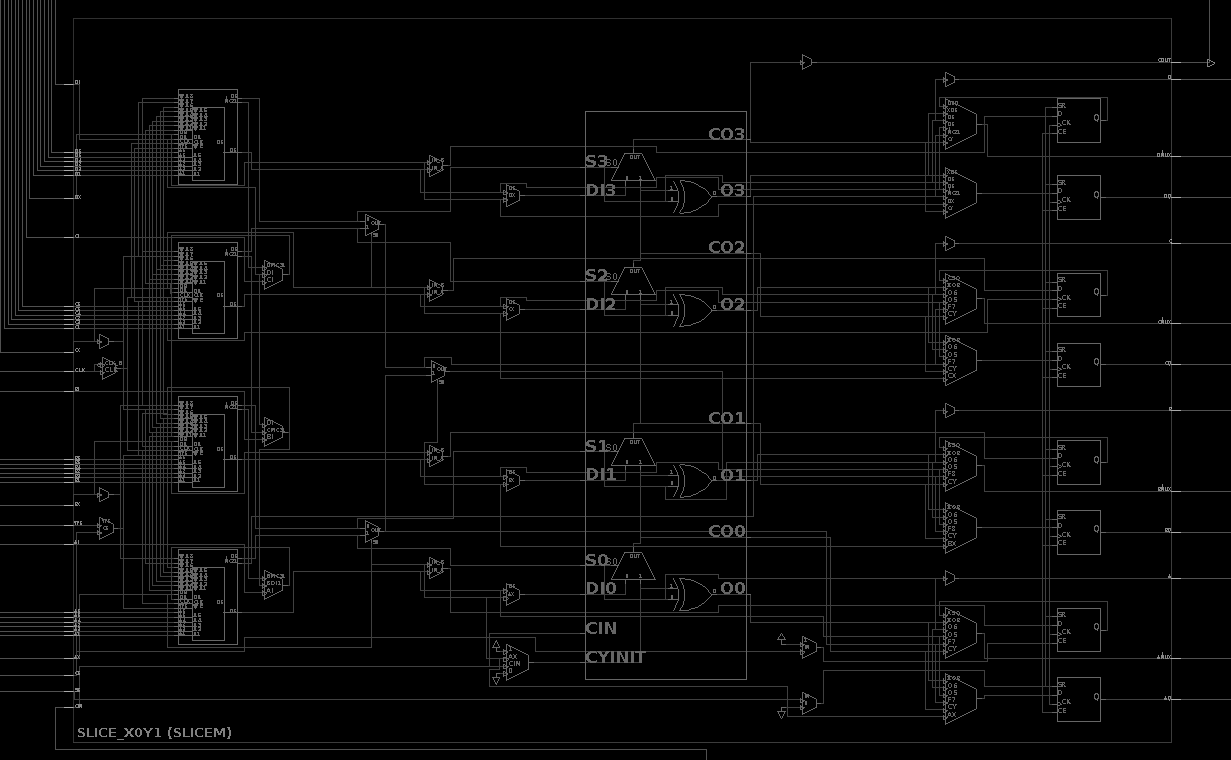
\includegraphics[width=\textwidth]{figures/slicem.png}
        \caption{SLICEM Site}
        \label{fig:slicem}
    \end{figure*}

    \begin{figure*}[t]
        \centering
        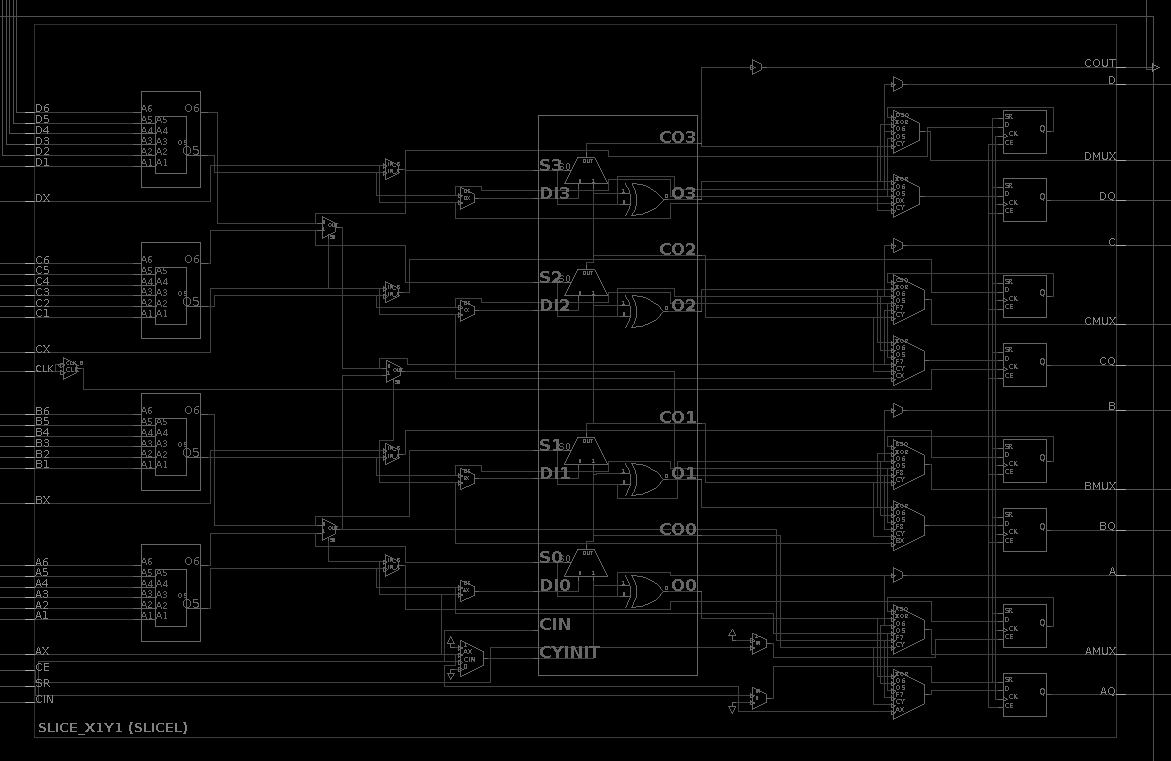
\includegraphics[width=\textwidth]{figures/slicel.png}
        \caption{SLICEL Site}
        \label{fig:slicel}
    \end{figure*}

\end{multicols}

\end{document}
